%%%%%%%%%%%%How does a GPS work and draw the state diagram for the GPS.Describe the different alternatives for measuring power consumption of a GPS%%%%%%%%%%%%%%%%%%%%%%%%%




\chapter{Theory}
\section{GPS}
The Global positioning system(GPS) is a space based radio navigation system developed by the Unites States Government, and has been operational since 1995.The system provides both timing and geolocation information to a GPS receiver anywhere on the Earth.  The system is not influenced by the number of receivers and can therefore serve an unlimited amount of users. The GPS system can deliver a position which is accurate within 22 meters horizontally if only one receiver is used. If multiple receivers is used positioning accuracy level of the order of a sub-centimeter to a few meters can be obtained \cite{GPS}. 

\subsection{Overview}
GPS consists three segments: space segment, control segment and the user segment. The space segment is a constellation of 24 satellites that are arranged so that  four to ten satellites is visible anywhere on the earth. Each satellite continuously broadcasts a signal composed of two carriers, two digital codes and a navigation message which contains the coordinates of the satellites as a function of the time. Each space vehicle as atomic clocks to ensure the integrity of the navigation message. The codes and the navigation message gets modulated with the two carrier frequencies.  \\If the distance between three satellites are known, the location of the receiver can be determined by measuring the angles with the respect of the each satellite.  GPS needs an additional satellite to account for the clock offset. Figure \ref{fig:GPS} shows the resection that is used by the satellites to determine the position.\\

\begin{minipage}[t]{0.8\textwidth}
\centering
    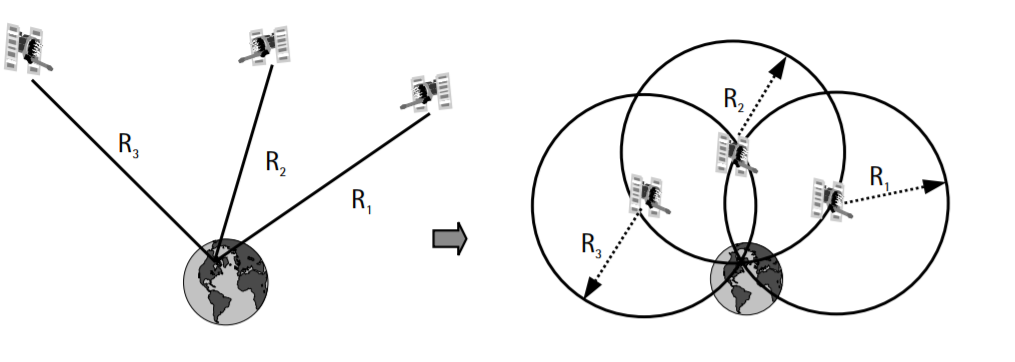
\includegraphics[width=0.8\textwidth]{Images/gps.PNG}\\
    \captionsetup{justification=centering}
    \captionof{figure}{Resection used by the satellites to determine the position}
    \label{fig:GPS}
\end{minipage}


 The distance between the satellite and the receiver are needed for using the method of resection.The Pseudorange is used for measuring the distance by assuming that the clock of the receiver and satellite are synchronized. It is called for pseudorange since they are actually not perfectly synchronized. The receiver can produce the digital codes at the same time instant that the satellites transmits them from space.The distance can be calculated by measuring the difference in delay of the transmitted signal from the produced one. The clocks is actually not perfectly synchronized and this is reason for the name pseudorange. \\
 A method for determining the velocity of a receiver is by estimating the Doppler frequency of the received signal. The Doppler shift is caused by the relative motion of the receiver and the SV. Figure \ref{modulation} shows the generated signals that are sent from each satellite. 
 
 \begin{figure}[H]
\centering
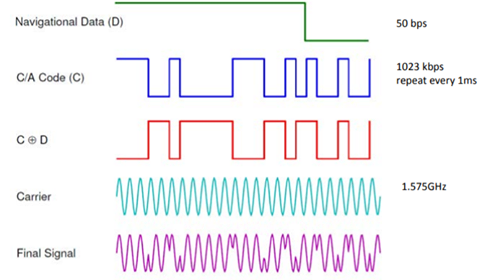
\includegraphics[width=16 cm]{Project_Report/Images/code_data.png}
\caption{The modulation of GPS signals}
\label{fig:modulation}
\end{figure}

 
 
 
 The two carrier frequencies L1 and L2 that the satellites transmits are generated at 1.5 MHz and 1,2 MHz respectively.  Each SV transmits the L1 and L2 signal but the code modulation for each is different to avoid interference. The two digital code coarse acquisition code (C/A) and precision code(P) consists of a stream of binary digits. The codes are generated using an algorithm and enables a receiver to distinguish the satellites since each have their own set of codes. The navigation message contains the ephemeris, the almanac, the health of the SV, the clock correction, and the atmospheric data.The Ephemeris is the precise information about the orbital position and clock correction for the specific satellite. The Almanac is a coarse orbital data of all the satellites in constellation. The Ephemeris is only valid for four hours and is sent every 30  second, while the Almanac is valid for 180 days and is sent every 12.5 minutes. \\
 The control segment of the GPS system consists of a number of world wide positioned tracking station and a master control station located in the United States. The control segment tracks the satellites to predict their location, control the atomic clock and satellite data that is transmitted by the SV. \\ The user segment is all GPS receivers that is used to determine their position.
  
  
 \subsection{Acquisition and Tracking}
  
The state diagram of a GPS receiver consists of two distinct phases, acquisition and tracking. Acquisition is the initial phase after start up. This is where the receiver searches and tries to detect the C/A codes from the satellites. After detecting and receiving satellite data from minimum four satellites the receiver starts the tracking phase.

After synchronizing the clock, the receiver determines the position and continues to search for other satellites signals. The receiver starts acquisition phase if it doesn't detect minimum four strong satellite signals.
Most receivers uses two separate engines for acquisition and tracking, the acquisition is usually the more power hungry of the two states.The time to first fix (TTFF) depends on three scenarios:
\begin{itemize}
\item Cold start: This is the same as a factory reset. The receiver doesn't have the last positional fix, the time or any satellite data of the constellation. Standard time to first fix  is about 1 minute.
\item Warm start: Last position,time and the Almanac is valid. The receiver does only have to download the Ephirems from the satellites. Standard estimation of TTFF is around 35s.
\item Hot start: When the previous fix was about one second ago, all the data is valid and the estimated time to next fix is 1 second. 

\end{itemize}




\newpage